\section{Problem formulation}
\label{sec:formulation}

\paragraph{Task}
A SHOW3D sample is one time instant of an egocentric recording observed by two synchronised, calibrated headset cameras $v\in\{0,1\}$ with pinhole intrinsics $\mathbf{K}_v$ and world-from-camera transforms $\mathbf{T}_{w\leftarrow v}=[\Rot_{w\leftarrow v}\,|\,\trans_{w\leftarrow v}]$~\cite{rim2026show3d,rim2026show3dapi}. For each hand $h\in\{L,R\}$ with joints $j=1,\dots,J$ ($J{=}21$ UmeTrack landmarks~\cite{han2022umetrack}), the target is the vector from the joint to the nearest vertex of the manipulated object,
\begin{align}
  \field_{h,j} &= \vtx_{m^*(h,j)}(\objpose) - \joint_{h,j},\label{eq:field}\\
  m^*(h,j) &= \arg\min_{m}\,\big\|\vtx_m(\objpose)-\joint_{h,j}\big\|_2.
\end{align}
where $\joint_{h,j}\in\mathbb{R}^3$ is the joint position, $\mesh_a=\{\vtx_m\}_{m=1}^{M_a}$ is the canonical mesh of the object with alias $a$, and $\vtx_m(\objpose)=\Rot_o\vtx_m+\trans_o$ are its vertices under the rigid pose $\objpose=(\Rot_o,\trans_o)$. Predictions are two $21\times 3$ arrays per frame in millimetres, expressed in the world frame. The world frame of SHOW3D is the frame of a body-mounted rig and changes over time, but the field is a difference of two points and is therefore translation invariant, so only the per-frame rotation $\Rot_{w\leftarrow c}$ of a reference camera $c$ is needed to move between camera and world frames. The object alias $a$ is part of the released test manifest and was used by the winning challenge entry~\cite{zou2026golf}; we treat it as an input. \Cref{fig:geometry} illustrates the geometry on a real frame.

\begin{figure}[t]
\centering
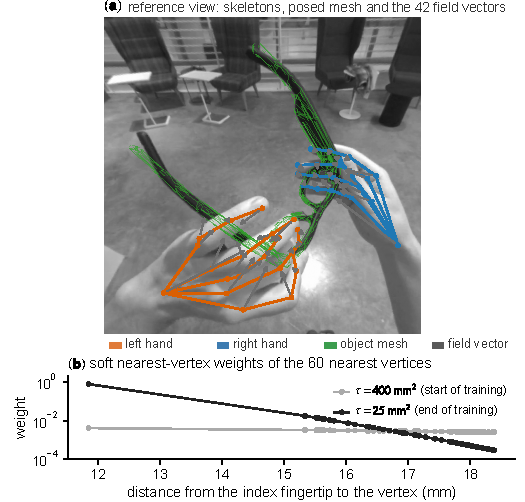
\includegraphics[width=\columnwidth]{../figures/fig3_field_geometry.pdf}
\caption{Geometry of the target on a SHOW3D training frame (subject ASC023 inspecting the glasses). (a) Projected skeletons, posed object mesh and the 21 nearest-vertex vectors of each hand in the reference view. (b) The soft nearest-vertex weights of \cref{eq:softw} for the index fingertip at the initial and final training temperature: at $\tau{=}400\,\mathrm{mm}^2$ the weight is spread over the local surface patch, at $\tau{=}25\,\mathrm{mm}^2$ it is concentrated on the nearest vertex.}
\label{fig:geometry}
\end{figure}

\paragraph{Evaluation}
The official evaluator reports, per directed field, the mean per-joint Euclidean endpoint error (ADE) over valid targets, the fraction of joints within 10, 50 and 100\,mm, and recall, the fraction of valid targets that received a prediction. A target is valid when the object pose and the hand pose are both confident (confidence above 0.5) and headset tracking succeeded~\cite{rim2026show3dapi}. We report the same quantities on held-out subjects and add the geometric and stratified measures of \cref{sec:setup}. Our re-implementation of the evaluator reproduces the organisers' code exactly.

\paragraph{The field is a derived quantity}
\Cref{eq:field} defines $\field_h=G(\joint_h,\objpose;\mesh_a)$ as a deterministic function of the hand joints, the object pose and a known mesh. Published solutions learn the composition $\mathrm{image}\mapsto\field$ end to end with a joint-query decoder~\cite{zou2026golf,jin2026jssr}; the geometric structure of $G$, in particular that all 21 endpoints of a hand lie on one rigid surface, is not used. Our method estimates the arguments of $G$ and applies $G$ itself. Two consequences follow. First, a prediction made through $G$ has endpoints on the object surface by construction, whatever the error in the arguments. Second, because $G$ depends on the posed surface only, it is invariant to the symmetry group of the object: the rotation of a can about its axis changes $\objpose$ but not $G$, so the object-pose branch need not resolve symmetric ambiguities that the field does not care about.

\paragraph{Falsification criterion}
Before any model was trained we fixed three predictions that the factored formulation has to meet, all at a matched frozen representation: (i) the factored model beats the direct head on mean ADE; (ii) the geometric supervision helps most on far-field and occluded joints; and (iii) transfer to a second dataset improves. The hypothesis is refuted if all three fail. The three clauses are tested in \cref{sec:main,sec:strata,sec:cross} respectively.
